%!TEX root = thesis.tex

\chapter{Approach}
\label{ch:approach}

\todo{Switching highest Priority, always first}

\section{Basic rules}
\todo{Game is turn based} \\
\todo{Each player has 6 Pokémon} \\
\todo{If a Pokémon has no HP left, it faints} \\
\todo{If all Pokémon of a player fainted, the player loses} 

\section{Battling}
\label{sec:battling}
One of the key aspects of the Pokémon game is to battle other Pokémon. In the mainline games, you can 
have up to six Pokémon in your team, also known as party. There is the option to swap a Pokémon with
another Pokémon, but you can't have more than six Pokémon at any point in your team. When playing the 
original Games, you can explore the world to find more Pokémon and use your team to defeat wild Pokémon
and other Pokémon trainer. This thesis however focus on random battles taking place on Pokémon Showdown.
In a random battle, both you and your opponent get a team of six random Pokémon. At the start of the battle,
you know each of your six Pokémon but only the currently active enemy Pokémon. \\
Every turn, both players can choose to either use a Move of their currently active Pokémon or switch
their active Pokémon to another Pokémon. Moves can either deal direct damage to the enemy Pokémon or 
yield other advantages like increasing the damage dealt by the next move. Moves will be covered in more
detail in section \ref{sec:moves}. Each Pokémon has an amount of \ac{HP}. The \ac{HP} of a Pokémon
can be dropped by attacking it with a Move. If the \ac{HP} of a Pokémon drops to zero, it faints and 
can't be used in this battle anymore. A player wins, if all Pokémon of the enemy are fainted. \\
\textit{Note:} In the mainline games there is the possibility to heal or even revive a fainted 
Pokémon during battle using \textit{Healing Items} like \textit{Revive} or \textit{Hyper Potion}.
In competitive Play, only \textit{Held items} like \textit{Leftovers} are allowed. Items will be explained
in depth in section \ref{sec:items}.

\subsection{Types}
\label{sec:types}
Pokémon implements a \textit{Rock-Paper-Scissors}-like system. Each Pokémon has eihter one or two of 
18 types. For example, a \textit{Fire}-type Pokémon is weak against \textit{Water}-type Pokémon
whereas a \textit{Water}-type Pokémon is weak against \textit{Grass}-type Pokémon. Lastly,
a \textit{Grass}-type Pokémon is weak against \textit{Fire}-type Pokémon. 
\begin{figure}
	\centering
	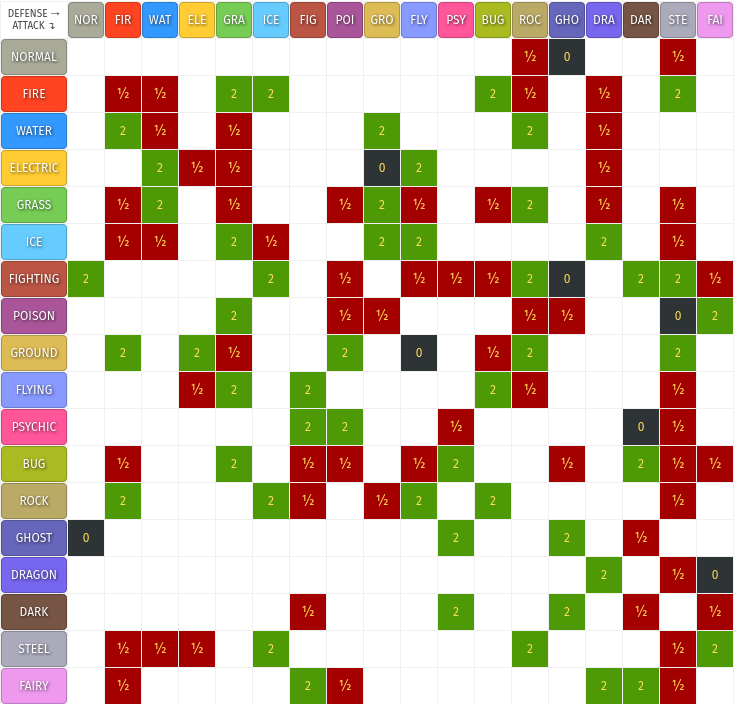
\includegraphics[width=0.7\textwidth]{images/type_chart.png}
	\caption{Pokémon type chart \cite{Pokemondb:Type}}
	\label{fig:type_chart}
\end{figure}
The figure \ref{fig:type_chart} shows how different Pokémon types interact with each other. It is important
to note, that the type modifiers will be multiplied if a Pokémon has two types. For example, a \textit{Fire}-type
attack will deal 4 times the damage against \textit{Parasect} as \textit{Parasect} has the types \textit{Grass} and
\textit{Bug} \cite{Veekun:Parasect}.

\subsection{Moves}
\label{sec:moves}
Moves can be split up into three categories: \textit{Physical}-, \textit{Special}- and \textit{Status}-Moves.
While \textit{Physical}- and \textit{Special}-moves usually deal damage to the opponent Pokémon, 
\textit{Status}-Moves can for example change the weather, which plays a role in damage calculation explained
in section \ref{sec:damage-calculation}, inflict status effects, raise or lower the stats of a Pokémon. Just 
as Pokémon, each Move has one of the 18 possible types. 

\subsection{Pokémon}
\label{sec:pokemon}
As stated in \ref{sec:battling}, each Pokémon has a given amount of \ac{HP}. However, two Pokémon of the same 
\textit{species}, meaning two Pokémon with the same name, can have different starting \ac{HP} values. The figure
\ref{fig:charizard-stats} shows the different \textit{stats} for the Pokémon \textit{Charizard}.
\begin{figure}
	\centering
	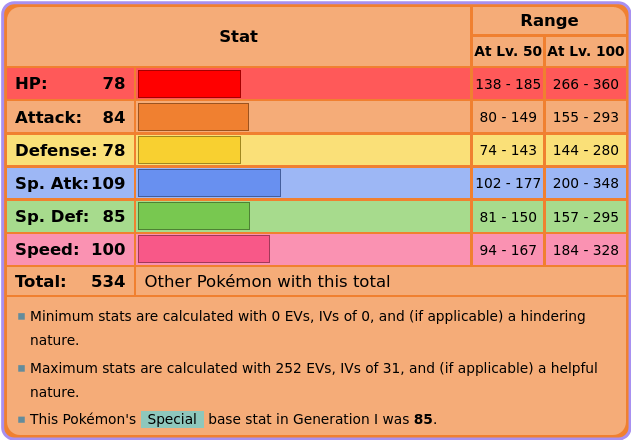
\includegraphics[width=0.7\textwidth]{images/charizard-stats.png}
	\caption{Charizard's stats \cite{Bulbapedia:Charizard}}
	\label{fig:charizard-stats}
\end{figure}
\paragraph{Explanation of stats}
\textbf{HP:} The \ac{HP} determines how much damage a Pokémon can receive before fainting. \\
\textbf{Attack:} The \ac{ATK} determines how much damage a Pokémon will deal when using 
a \textit{Physical}-Move. \\
\textbf{Defense:} The \ac{DEF} determines how well a Pokémon can resist against physical attacks. \\
\textbf{Sp. Atk:} The \ac{SPA} determines how much damage a Pokémon will deal when using
a \textit{Special}-Move. \\
\textbf{Sp. Def:} The \ac{SPD} determines how well a Pokémon can resist against special attacks. \\
\textbf{Speed:} The \ac{SPE} determines how fast a Pokémon can act. This is important as instead of
both Pokémon moving at the same time, the Pokémon with the higher \ac{SPE} will move first. After 
the faster Pokémon moved, the slower Pokémon will move. Therefore, the faster Pokémon is usually at an
advantage. 
\todo{Cover priority moves and trickroom}
\todo{Cover evasion / accuracy, context to showdown}
\paragraph{Status condition}
A Pokémon can have a status condition, this affects the Pokémon negatively. Status conditions are
inflicted by moves. The most important status conditions are
\begin{itemize}
	\item \textbf{Burn:} If a Pokémon suffers from the status condition \ac{BRN}, it will lose 1/8 of its
		total \ac{HP} every turn. In addition to that, a burned Pokémon will only deal half as much damage
		when using a \textit{physical} move.
	\item \textbf{Freeze:} If a Pokémon suffers from the status condition \ac{FRZ} it won't, with a few exceptions,
		be able to use moves
	\item \textbf{Paralysis:} If a Pokémon suffers from the status condition \ac{PAR} it won't be able to use 
		the selected move 25\% of the time and their Speed is halved.
	\item \textbf{Poison:} If a Pokémon suffers from the status condition \ac{PSN} it will, with a few exceptions,
		take damage equal to 1/8 of its total \ac{HP} at the end of every turn. A Pokémon can also be 
		\textit{badly poisoned}. Badly poison initially inflicts damage equal to 1/16 of the Pokémon's maximum
		\ac{HP}, with the damage inflicted increasing by 1/16 each turn. This means that the Pokémon will
		take 2/16 damage on the second turn, 3/16 on the third turn.
	\item \textbf{Sleep:} If a Pokémon suffers from the status condition \ac{SLP} it won't be able to use moves,
		except \textit{Snore} and \textit{Sleep Talk}. In the mainline games, sleep lasts randomly between
		one and three turns. However, in Pokémon Showdown a Pokémon will \textit{always} be asleep for exactly
		two turns.
\end{itemize}

At any point, a Pokémon can only suffer from one status condition at a time, this means that a 
\textit{burned} Pokémon can't fall asleep.

\paragraph{Determination of stats}
\label{sec:stat-calculation}
The total stat of a Pokémon is calculated as described in equation \ref{eq:stats-hp} and equation 
\ref{eq:stats-other} \cite{Bulbapedia:Stat}.
\begin{equation}
	\label{eq:stats-hp}
	HP = \Bigl\lfloor \frac{(2 \times Base + IV + \lfloor \frac{EV}{4} \rfloor) \times Level}{100}\Bigr\rfloor
	+ Level + 10 \\
\end{equation}
\begin{equation}
	\label{eq:stats-other}
	OtherStat = \Bigl\lfloor \Big( \frac{2 \times Base + IV + \lfloor \frac{EV}{4} \rfloor) \times Level}
	{100} + 5\Big) \times Nature \Bigr\rfloor
\end{equation}
\textbf{Base:} Refers to the base stat of a Pokémon. Two Pokémon of the same species will always have the 
same base-stats. As seen in figure \ref{fig:charizard-stats}, a \textit{Charizard} will always have a
base-\ac{ATK} of 84.

\textbf{Level:} As mentioned in section \ref{sec:battling}, the goal of the mainline games is to create 
a team of six Pokémon and to make that team stronger by fighting other Pokémon. If a Pokémon defeats
enough other Pokémon, it grows a Level. The maximum level of a Pokémon is 100. If the level of a Pokémon
increases, so will its stats. For each level gained (ignoring Nature), stats will increase by 1/50 the
base stat value, and 1/100 the combined \ac{IV} and \ac{EV} values \cite{Bulbapedia:Stat}. 
In Pokémon Showdown, the level of  a Pokémon is set at the start of the battle and won't 
increase \cite{Smogon:RandBatsGuide}.

\textbf{Nature:} A Pokémon has a nature. Most natures enhance the growth of one stat, while hindering
the growth of another. After all other calculations are finished, the stat that the Nature enhances will
be 100\% of what it would be without the Nature, and the stat hindered will be 90\% of its normal value
\cite{Bulbapedia:Stat}. Nature can be neglected in this thesis as all Pokémon in random battles have
a neutral nature, meaning no stat is enhanced or hindered \cite{Smogon:RandBatsGuide}.

\textbf{IV:} Refers to the \ac{IV} of a Pokémon. These cause two Pokémon of the same species to have
different Stats \cite{Bulbapedia:Stat}. Pokémon in Pokémon Showdown will always have the best possible \ac{IV} 
stat, 31, unless it is a disadvantage for the Pokémon, then it will be zero \cite{Smogon:RandBatsGuide}.

\textbf{EV:} These are the \ac{EV} of the Pokémon. \ac{EV} are what causes a trained Pokémon to have higher
stats than an untrained counterpart of the same level. For every 4 \ac{EV} gained, a level 100 Pokémon 
will have 1 extra point in the given stat. A Pokémon can earn up to 510 \ac{EV}, but can't have more than
255 \ac{EV} in a single stat \cite{Bulbapedia:Stat}. Random Pokémon on Showdown will always have 85 
\ac{EV} in each stat, or 0 in the case that having a high stat being detrimental \cite{Smogon:RandBatsGuide}.

\subsection{Switching}
\label{sec:switching}
Instead of using a move with the current Pokémon, the player also has the option to switch out the 
active Pokémon for another Pokémon is his party. Switching always takes place before the execution of moves.
However, the player does not know whether the opponent is switching or using a Move. Therefore, if the 
player decides to switch out a non-fainted Pokémon, the enemy gets to use his move on the new Pokémon.
If a Pokémon faints, the player has to switch in a new Pokémon and then the next turns tarts. This means
that the opponent gains a one turn advantage if the player decides to switch out a healthy Pokémon, but
won't get to attack an additional time if the Pokémon was defeated.  

\subsection{Items}
\label{sec:items}
A Pokémon can also hold an Item that yields benefits in battle. There are various purposes that items 
can fulfill. For example, the item \textit{Life Orb} boosts damage dealt by the holder's damaging move
by 30\%\footnote{This boost is approximated as 5324/4096 $\approx$ 1.29980}, but the holder takes
damage equal to 10\% of its maximum \ac{HP} after it uses a damaging move\footnote{Rounded down, 
but not less than 1} \cite{Bulbapedia:LifeOrb}. \textit{Leftovers} restore 1/16 of the holder's
maximum \ac{HP}\footnote{Rounded down, but not less than 1} at the end of each turn whereas the item
\textit{Air Balloon} makes the holder \textit{ungrounded}, which means that the holder is immune to
\textit{Ground}-type moves as well as several related effects\cite{Bulbapedia:AirBalloon}. The 
items generated in Pokémon Showdown are described in more details in \ref{sec:randbats-items}.
\paragraph{Important items}
\label{sec:Important-items}
In this section, a quick introduction to the most important items is given.
\begin{itemize}
	\item \textbf{Choice Band:} When held by a Pokémon, this item boosts the \ac{ATK} by 5ß\%, but only
	allows the use of the first move selected. This effect resets when the holder is switched out \cite{Bulbapedia:ChoiceBand}. 
	\item \textbf{Choice Scarf:} When held by a Pokémon, this item boosts the \ac{SPE} by 5ß\%, but only
	allows the use of the first move selected. This effect resets when the holder is switched out \cite{Bulbapedia:ChoiceScarf}. 
	\item \textbf{Choice Specs:} When held by a Pokémon, this item boosts the \ac{SPA} by 5ß\%, but only
	allows the use of the first move selected. This effect resets when the holder is switched out \cite{Bulbapedia:ChoiceSpecs}. 
	\item \textbf{Leftovers:} Restores 1/16 of the holder's maximum \ac{HP} at the end of each turn \cite{Bulbapedia:Leftovers}.
	\item \textbf{Life Orb:} Boosts the damage dealt by the holder's damaging moves by 30\%, but the holder takes damage 
	equal to 10\% of its maximum \ac{HP} after it uses a damaging move \cite{Bulbapedia:LifeOrb}.
	\item \textbf{Heavy-Duty Boots:} The holder is unaffected by the effects of entry hazards. Entry hazards are described 
	in \ref{sec:hazards}. If a \textit{grounded} \textit{Poison}-type Pokémon enters the field while holding this item,
	it will cause \textit{Toxic Spikes} to be removed \cite{Bulbapedia:HeavyDutyBoots}.
	\item \textbf{Assault Vest:} Raises the holders \ac{SPD} by 50\%, but also prevents the holder from selecting any 
	status move\footnote{Except \textit{Me First}} \cite{Bulbapedia:AssaultVest}.
	\item \textbf{Focus Sash:} If the holder has full \ac{HP} and is hit by an attack that would otherwise cause fainting,
	it survives with 1 HP \cite{Bulbapedia:FocusSash}.
\end{itemize}

\subsection{Field effects}
There are multiple \textit{field effects} that affect combat.
\paragraph{Terrain}
\textit{Terrain} is set up by the respective move with identical name and last for five turns. 
All of them are beneficial to \textit{grounded} Pokémon. A Pokémon is \textit{not grounded} if any of the 
following conditions apply:
\begin{itemize}
	\item The Pokémon has the \textit{Flying}-type
	\item The Pokémon has the Ability Levitate
	\item The Pokémon is holding the item \textit{Air Balloon}
	\item The Pokémon is under the effect of \textit{Magnet Rise} or Telekinesis.
\end{itemize}
\textit{Grounded} Pokémon are with a few exceptions those Pokémon, that are not \textit{ungrounded}. A 
Pokémon will be grounded if any of the following conditions apply:
\begin{itemize}
	\item The Pokémon is holding an \textit{Iron Ball}
	\item The Pokémon is under the effect of \textit{Ingrain}, \textit{Smack Down} or \textit{Thousand Arrows}.
	\item The \textit{Field effect} \textit{Gravity} is in effect.
\end{itemize}
More information about grounding can be found at \cite{Bulbapedia:Grounded}
There are five different possible \textit{terrain}-states. 
\begin{itemize}
	\item \textbf{None:} The default state, no other effects are applied. 
	\item \textbf{Electric Terrain:} Grounded Pokémon can't fall asleep and the power of \textit{Electric}-type
		moves is also by 50\%.
	\item \textbf{Grassy Terrain:} The HP of grounded Pokémon is restored by 1/16 of their maximum HP at the
		end of each turn. In addition, the power of \textit{Grass}-type moves is increased by 50\% and the 
		moves \textit{Earthquake}, \textit{Magnitude} and \textit{Bulldoze} halve in power. 
	\item \textbf{Misty Terrain:} protects all grounded Pokémon from status conditions (including confusion).
		The power of \textit{Dragon}-type moves is halved while in effect. 
	\item \textbf{Psychic Terrain} prevents grounded Pokémon from being hit by high-priority moves (such as
		\textbf{Quick Attack} or \textit{Sucker Punch}). The power of \textit{Psychic}-type moves is also increased
\end{itemize}
It is important to note, that only one \textit{terrain} can be active at a time, yet, \textit{terrain}
can coexist with other \textit{field effects} like \textit{weather}.

\paragraph{Weather}

\subsection{Damage calculation}
\label{sec:damage-calculation}
The damage dealt by a move mainly depends on the \textit{level} of the Pokémon
that uses the move, its effective Attack or Special Attack stat, the
opponent's effective Defense or Special Defense stat and the move's effective
power. 

Precisely, the damage is calculated as follows\cite{Bulbapedia:Damage}:
\begin{dmath}
  \text{Damage} = \left(\frac{\left(\frac{2 \times \text{Level}}{5}\right) \times \text{Power} \times \text{A / D}}{50} + 2\right)
	\times Targets
	\times Weather
	\times Badge
	\times Critical
	\times random
	\times STAB
	\times Type
	\times Burn
	\times other
\end{dmath}

The only exception for this are moves that deal direct damage. A list 
of these moves can be found at \cite{Bulbapedia:DirectDamage}.

\paragraph{Level}
\textit{Level} refers to the level of the attacking Pokémon\cite{Bulbapedia:Damage}. 
In Pokémon Showdown, the level is displayed next to the name of the Pokémon.
\todo{Mainline games leveling}

\paragraph{A / D}
\textit{A} is the effective Attack stat of the attacking Pokémon if the used move is a physical move,
\todo{Reference to physical moves} \\
or the effective Special Attack stat of the attacking Pokémon if the used move is a special move.
\todo{Reference to special moves}
\\
\textit{D} is likewise the effective Defense stat of the target if the used move is a physical move,
or the effective Special Defense of the target if the used move is a special move\cite{Bulbapedia:Damage}.

There are four moves that use stats from different categories, more Information can be found
at \cite{Bulbapedia:MoveStatDifferentCategories}.

\paragraph{Power}
Power is the effective power of the used move.
\todo{When is the power not equal to the base power}
The \textit{Base Power} of a move in Showdown can be seen when hovering over a move in the move list. \\
\textit{Note:} The same move will always have the same base power. For example, \textit{Fire Punch} will
always have a base power of 75\cite{Bulbapedia:FirePunch}.

\paragraph{Weather}
The \textit{Weather} modifier is 1.5 if a \textit{Water-type} move is used during \textit{rain} or a 
\textit{Fire-type} move during \textit{Harsh Sunlight}. The modifier is 0.5 if a \textit{Water-type} move
is used during \textit{Harsh Sunlight} or a \textit{Fire-type} move during \textit{rain} \cite{Bulbapedia:Damage}.
\todo{Reference to weather section}

\paragraph{Critical}
In the latest Generation, a \ac{CRIT} deals 1.5 times the damage compared to a normal hit.
If the \ac{CRIT} rate is not increased, the chance of landing a \ac{CRIT} is 1/24
\cite{Bulbapedia:CriticalHit}. Increasing \ac{CRIT} rate, as well as other stats, will 
be explained in chapter \ref{sec:boosting}. \\
\textit{Note:} In earlier games, \ac{CRIT}s worked different, see \cite{Bulbapedia:CriticalHit} for
more details.

\paragraph{Random}
\textit{Random} is a random integer percentage between 85\% and 100\%. Because of this, the same move
may deal different damage in the same scenario \cite{Bulbapedia:Damage}.

\paragraph{STAB}
\textit{STAB} stands for \textit{Same Type Attack Bonus}. It is a multiplier of 1.5 if the used move
is of the same type as the attacking Pokémon. Otherwise, it is 1.0 \cite{Bulbapedia:Damage}.

\paragraph{Type}
This is the in section \ref{sec:types} described type modifier \cite{Bulbapedia:Damage}.

\paragraph{Burn}
\textit{Burn} is 0.5 if the attacking Pokémon is burned, and the used move
is a physical move\footnote{This does not apply if the attacking Pokémon has the Ability \textit{Guts}
or the used move is \textit{Facade}}. Otherwise, it is 1.0 \cite{Bulbapedia:Damage}.

\paragraph{Other}
The \textit{other} modifier is usually 1. A list of exceptions can be found at \cite{Bulbapedia:Damage}.

\subsection{Effective Stats}
\paragraph{Boosting}
\label{sec:boosting}
\todo{Boosting critical rate}

\section{Hazards}
\label{sec:hazards}
An \textit{entry hazard} is a condition that affects a side of the field that causes
any Pokémon that is sent into battle on that side of the field to be afflicted by 
a negative effect. Entry hazards are created by moves, usually status moves
\cite{Bulbapedia:EntryHazards}. \\
\todo{This paragraph is copied word by word from Bulbapedia}
\subsection{List of entry hazards}
Currently, there are five moves that create an entry hazard

\paragraph{Spikes}
\textit{Spikes} is a \textit{Ground}-type entry hazard that causes the opponent
to lose $1/8$\% of their maximum \ac{HP} when they enter the field. This
effect can be stacked up to three times. Two layers of spikes will deal
$1/6$\% and three layers will deal $1/4$\% of the enemies maximum \ac{HP}. \\
\todo{Removal and Immunity of Spikes}
Spikes are created by the move \textit{Spikes}\cite{Bulbapedia:Spikes}.

\paragraph{Stealth Rock}
\label{sec:stealthrock}
The move \textit{Stealth Rock} sets an entry hazard around the target Pokémon
causing Pokémon on the target's field to receive damage upon being switched in.
The amount of damage inflicted is affected by the effectiveness of the type
\textit{Rock} against the target. Unlike Spikes, this entry hazard does not stack.
The damage taken from the victim's maximum is denoted in table 
\ref{tab:stealth-rock-damage}\cite{Bulbapedia:StealthRock}.
\begin{table}[h]
	\label{tab:stealth-rock-damage}
	\centering
	\begin{tabular}{|c|c|}
		\hline
		\textbf{Type effectiveness} & \textbf{Damage (Max. \ac{HP}}) \\
		\hline 
		0.25x & 3.125\% \\ 
		\hline 
		0.5x &  6.25\% \\ 
		\hline 
		1x & 12.5\% \\
		\hline
		2x & 25\% \\
		\hline
		4x & 50\% \\
		\hline
	\end{tabular} 
	\caption{Damage dealt to Pokémon by Stealth Rocks\cite{Bulbapedia:StealthRock}}
\end{table}
\textit{Note:} Stealth Rocks can also be created by the move \textit{G-Max Stonesurge}.
This damage-dealing Water-type G-Max move is exclusive to Gigantamax Drednaw
\cite{Bulbapedia:GMaxStonesurge}. \\
\todo{Does this move exist in Showdown}

\paragraph{Sticky Web}
The entry hazard set by the \textit{Bug}-type move \textit{Sticky Web} lowers the
opponents speed stat by one stage upon switching in \cite{Bulbapedia:StickyWeb}. \\
\todo{Pokémon that are not affected by this}

\paragraph{Poison spikes}
\label{sec:poison-spikes}
\textit{Poison Spikes} set by the \textit{Poison}-type move \textit{Toxic Spikes}
cause the opponent to become poisoned. If two layers of spikes are set, the
Pokémon instead becomes badly poisoned \cite{Bulbapedia:ToxicSpikes}. \\
\todo{Pokémon not affected} \\
\todo{Explain (badly) poisoning}

\paragraph{Sharp steel}
This entry hazard works very similar to Stealth Rock described in \ref{sec:stealthrock}.
However, Sharp steel can only be set by the \textit{Steel}-type move
\textit{G-Max Steelsurge} which is the exclusive G-Max Move of Gigantamax Copperhead.
The damage dealt by Sharp steel does not stack, the amount of damage dealt is
based on the Type effectiveness of the \textit{Steel}-type against the target.
Exact damage modifiers can be found in table \ref{tab:sharp-steel-damage}
\cite{Bulbapedia:GMaxSteelsurge}.
\begin{table}[h]
	\label{tab:sharp-steel-damage}
	\centering
	\begin{tabular}{|c|c|}
		\hline
		\textbf{Type effectiveness} & \textbf{Damage (Max. \ac{HP}}) \\
		\hline 
		0.25x & 3.125\% \\ 
		\hline 
		0.5x &  6.25\% \\ 
		\hline 
		1x & 12.5\% \\
		\hline
		2x & 25\% \\
		\hline
		4x & 50\% \\
		\hline
	\end{tabular} 
	\caption{Damage dealt to Pokémon by Sharp Steel\cite{Bulbapedia:GMaxSteelsurge}}
\end{table}
\todo{Unaffected Pokémon}

\subsection{Hazard counterplay}
There are some moves that can remove entry hazards. \textit{Rapid Spin} 
\cite{Bulbapedia:RapidSpin} removes entry hazards from the user's side of the field and
\textit{Defog}\cite{Bulbapedia:Defog} removes entry hazards on both sides of the 
field\footnote{In older games \textit{Defog} would only remove Hazards on the
target's side of the field. But as we only investigate the latest version, this
won't be covered in detail.}. In addition, 
\textit{Court Change}\cite{Bulbapedia:CourtChange} will exchange the entry hazards
on each side of the field, along with other one-sided field conditions.
\todo{What other one-sided field conditions are there?}
If a grounded\footnote{The term \textit{grounded} is used to describe a Pokémon that
can't be affected by damaging \textit{Ground}-type moves and several other associated 
effects\cite{Bulbapedia:Grounded}.}
\textit{Poison}-type Pokémon enters the battle, it will remove Toxic 
Spikes, described in \ref{sec:poison-spikes}, from its side of the field.
Lastly, Pokémon holding the item 
\textit{Heavy-Duty Boots}\cite{Bulbapedia:HeavyDutyBoots} are unaffected by
entry hazards, but grounded \textit{Poison}-type Pokémon can still remove
Toxic Spikes even if they hold the boots\cite{Bulbapedia:EntryHazards}.
There are various exceptions and special cases to hazards. 
\todo{Special cases of hazards}

\section{Showdown random battles}
\todo{Write introduction to this}
\todo{This has to include that the same species has different movesets}
\label{sec:showdown-randbats}
\subsection{Sets}
\label{sec:randbats-sets}
As described in section \ref{sec:stat-calculation}, Pokémon created for random battles
usually have 85 \ac{EV}s and 31 \ac{IV} in every stat with a neutral nature, 
meaning a nature that does neither boost nor hinder any stat \cite{Smogon:RandBatsGuide}.
There are some cases where a high stat is not beneficial, an example would be the 
move \textit{Gyro Ball}. Unlike most moves, the \textit{Base Power} of this move
described in the damage calculation described in \ref{sec:damage-calculation} is not
a fixed value. It is determined as described in \ref{eq:gyroball-base-power} \cite{Bulbapedia:GyroBall}.
\begin{equation}
	\label{eq:gyroball-base-power}
	BasePower = \min(150, \frac{25 \times CurrentSpeed_{target}}{CurrentSpeed_{user}})
\end{equation} 
As the damage dealt by \textit{Gyro Ball} gets bigger, the lower the \ac{SPE} of the
attacker, Pokémon using this move have 0 \ac{EV} and 0 \ac{IV} in the \ac{SPE} stat. \\
\textit{Note:} Being able to outspeed the opponent is extremely valuable, but the only
two Pokémon using \textit{Gyro Ball}, \textit{Stakataka} and \textit{Ferrothron}, already
have a very low \ac{SPE} stat and are slower than almost all other Pokémon in random
battles. A complete list of Pokémon with their respective \ac{SPE} stat can be found
at \cite{Bulbapedia:PokemonBySpeed}. \\
This knowledge can be exploited to gather additional information about the enemy, section
\ref{sec:builds-randbats} describes how this is achieved.

\subsection{Items}
\label{sec:randbats-items}
Items in random battles are procedurally generated by showdown and depend on the Pokémon's
moves, base stats and ability. As stated in \cite{Smogon:RandBatsGuide}, the exact implementation
is \glqq changed frequently with the intention of optimizing set generation\grqq, yet, item
assignment follows these rules:
\begin{itemize}
	\item Pokémon with 2 or fewer attacking moves will get \textit{Leftovers}, or 
	\textit{Black Sludge} if \textit{Poison}-type.
	\item Pokémon with 3 attacking moves will get \textbf{Life Orb}, if the sum of their base
	\ac{HP}, \ac{DEF} and \ac{SPD} is less than 275. Otherwise, these Pokémon get 
	\textit{Leftovers} or \textit{Black Sludge}.
	\item Pokémon with 4 matching attacks get a \textit{Choice} item which follows these rules:
	\begin{itemize}
		\item Pokémon with four physical attacks or four special attacks, a base \ac{SPE} between
		60 and 108 and base \ac{ATK} or \ac{SPA} of 100 or more can get a \textit{Choice Scarf}
		2/3 of the time. If the Pokémon doesn't meet one of the stat qualifications or doesn't
		get the 2/3 chance, they'll get \textit{Choice Specs} or \textit{Choice Band} instead.
		\item Pokémon with 3 special attacks and the move \textit{U-turn} always get 
		\textit{Choice Specs}. \textit{U-turn} is a physical, \textit{Bug}-type move that 
		switches the user out after damage is dealt \cite{Bulbapedia:UTurn}.
		\item Pokémon with \textit{Trick} \cite{Bulbapedia:Trick} or \textit{Switcheroo} 
		\cite{Bulbapedia:Switcheroo}, both moves that allow to switch items
		with the opponent, they will always get a choice item. If they meet the above-mentioned 
		speed range, they will always get a \textit{Choice Scarf}. Otherwise, they will always
		get \textit{Choice Specs} or \textit{Choice Band}.
		\item Having priority moves will always prevent a \textit{Choice Scarf} from being 
		generated in all situations.
		\todo{Either explain priority moves or explain them here}
	\end{itemize}
	\item Pokémon with 4 attacks that don't qualify for choice items, will get an \textit{Assault
	Vest} if their \ac{HP} + \ac{DEF} + \ac{SPD} $\geq$ 235. Otherwise, \textit{Expert Belt},
	\textit{Leftovers} or \textit{Life Orb} is generated.
	\item Pokémon that are weak to Rock will get \textit{Heavy-Duty Boots} if they don't get a 
	higher priority item, such as \textit{Assault Vest} or a choice item. Pokémon that are four
	times weak to \textit{Rock}, such as \textit{Charizard}, will always get \textit{Hevay-Duty Boots}.
	This is done as these Pokémon would otherwise loose up to 50\% \ac{HP} to the entry hazard
	\textit{Stealth Rock} described in \ref{sec:stealthrock}. The only exception is \textit{Scyther},
	which can get Eviolite.
	\item Pokémon in the lead slot will get \textit{Focus Sash} if their \ac{HP} + \ac{DEF} + \ac{SPD} < 255,
	and they would otherwise get \textit{Leftovers} or \textit{Life Orb}.
	\item Pokémon that get a Speed-boosting move will be given a \textit{Weakness Policy} if their \ac{HP}
	+ \ac{DEF} + \ac{SPD} $\geq$ 300, and they aren't four times weak to \textit{Ground}. This item
	boosts the \ac{ATK} and \ac{SPA} by two stages each if hit by a super effective move. After that,
	the item breaks \cite{Bulbapedia:WeaknessPolicy}.
\end{itemize}
There are also some species that will always roll the same item, either because it's their signature item or
because doing so supports a niche ability or set. For example, Pikachu always has \textit{Light Ball}

\section{Pokémon Matchups}
Due to the typing system, there is no best Pokémon that is the best option in all situations. Therefore, we 
have to determine how good a Pokémon is against another Pokémon in a given situation. In this case, the
\textit{situation} refers to the current state of both Pokémon like current \ac{HP} and status conditions
as well as field effects like weather. 
\subsection{Check and Counter}
There are multiple definitions of \textit{check} and \textit{counter} \todo{Cite multiple definitions}. In
this thesis, we refer to a Pokémon \textit{checking} another Pokémon if it can beat the enemy Pokémon in 
every scenario and can safely be switched in at any point. A \textit{counter} is also capable of defeating
the enemy Pokémon but may lose in some situations. The most notable being if switched in without the
previous active Pokémon fainting as this grants the opponent an additional attack. \\
The key difference between \textit{check} and \textit{counter} is, that a check is also stronger if
it takes damage once more while a counter is not guaranteed to win in this situation. \\
\textit{Note:} Every \textit{check} to a Pokémon is also always a \textit{counter} while \textit{counter}
could also be a \textit{check}, but is not guaranteed to. 

\section{Implementation}
\subsection{Communication with Pokémon Showdown}
\label{sec:poke-env}
The communication with Pokémon Showdown is handled using the python library \textit{Poke-Env} \cite{PokeEnv:Github}.
This library provides a lot of the core functionality needed, like accessing the current Pokémon in battle as well
as switch and move options. However, it does not provide functionality for damage calculation. We use the \textit{Pokémon
Damage Calculator} \cite{Smogon:DamageCalc}, a node library written by the smogon-team for that. 
Communication between the two libraries is implemented by capturing stdout and stdin using the \textit{subprocess} python library.

\subsection{Gathering Information about the enemy Pokémon}
\label{sec:builds-randbats}
As mentioned in \ref{sec:showdown-randbats}, the same Pokémon can occur in various different builds, meaning the combination
of moves, abilities and items. Knowing the exact enemies build is very important for decision-making. Consider the following
example: 
\begin{itemize}
	\item \textbf{Player1} has an active \textit{Charizard} with \textit{Heavy-Duty Boots} and 150\ac{HP} remaining on the field.
	\item \textbf{Player2} has just sent out a \textit{Drapion} with 160\ac{HP} remaining.
	\item The \textit{Charizard} is faster but can't kill the enemy \textit{Drapion} in one turn as his move 
	\textit{Fire Blast} deals between 127 and 151 damage to the \textit{Drapion}. 
	\item Therefore, if \textbf{Player1} decides to attack, \textit{Drapion} is guaranteed to survive this turn
	and can attack \textit{Charizard} as well.
\end{itemize}
In this scenario, the optimal play for \textbf{Player1} depends heavily on the move set of the enemy \textit{Drapion}.
Possible moves for \textit{Drapion} are:
\begin{itemize}
	\item \textit{Aqua Tail}: A damaging \textit{Water}-type move
	\item \textit{Earthquake}: A damaging \textit{Ground}-type move
	\item \textit{Knock Off}: A damaging \textit{Dark}-type move
	\item \textit{Poison Jab}: A damaging \textit{Poison}-type move
	\item \textit{Swords Dance}: A move to raise the own \ac{ATK} by two stages
	\item \textit{Taunt}: A move that makes the afflicted Pokémon unable to use status moves
	\item \textit{Toxic Spikes}: A move that sets an entry hazard.
\end{itemize}
Hereby it is important to note, that \textit{Drapion} only knows the move \textit{Aqua Tail}, if it knows four total 
damaging moves. In the given scenario, \textbf{Player1} should switch out his \textit{Charizard} if the enemy
\textit{Drapion} knows the move \textit{Aqua Tail} as this attack would kill \textit{Charizard}. We can determine 
whether the enemy knows \textit{Aqua Tail} based on his item:
\begin{itemize}
	\item If \textit{Drapion} rolls two status moves, it will have the item \textit{Black Sludge} and therefore 
	doesn't know \textit{Aqua Tail}. Because \textit{Drapion} is already damaged, we know that it has this item
	if it healed 1/16\% of his max \ac{HP} in his last turn. 
	\item If \textit{Drapion} rolls one status move, it will have the item \textit{Life Orb}. If \textit{Drapion}
	already attacked, we know if it has a \textit{Life Orb} or not as this item causes it to lose 10\% of his
	maximum \ac{HP} after an attack.
	\item If \textit{Drapion} has neither \textit{Black Sludge} nor \textit{Life Orb}, it has to have a
	\textit{Choice Band} and as this item will only generate if the Pokémon knows four matching attacks,
	and therefore has to know the move \textit{Aqua Tail}.
\end{itemize}
\paragraph{Implementation details}
The first step to predicting enemy sets is to determine all possible sets as well has how likely each individual set
is. In order to achieve this, I wrote a script that to start a battle between an information gathering player and 
a random agent. In the next step, the script extracts all builds of all Pokémon and stores them, then, it forfeits, 
and a new battle is started. Once enough battles are played, the script will store the builds as well as how often
they appeared in text files, one file for each Pokémon. \\
In actual battles, if a new Pokémon enters the enemy side, we assume it to have the most likely build for this species. 
Once more information becomes available on items, moves and abilities, we rule-out non-matching builds and always
assume the enemy to have the remaining most likely build.

\subsection{Scoring the current game state}
In Order to not only rate the current board state, but also individual Pokémon, we implement the following scoring 
algorithm:
\begin{equation}
\label{eq:score-attack}
	score(e_{i, j}) = \text{Expected Damage that Pokémon } i \text{ will deal to Pokémon j}
\end{equation}
The expected damage is the damage dealt if both Pokémon behave optimal in the amount of turns that the bot looks into
the future. Section \ref{sec:determine-matchups} covers how the optimal moves are determined.
\ref{eq:score-attack}
\begin{equation}
	val(i) = \sum_{j \in \text{Enemy Pokémon}} score(e_{i, j})
\end{equation}
Using this, we can also introduce a \textit{value} for each of our Pokémon where a higher value implies a more important
Pokémon. It is important to note, that scores are determined independently of each other meaning that we do not take
into account damage taken by the attacker. This does explicitly mean that this metric does not determine how good the 
Pokémon is if it has to battle \textit{all} enemy Pokémon but rather against how many other Pokémon it \textit{could}
be used. This is done as the order in which a Pokémon battles multiple Pokémon plays a huge role. The reasoning
behind this as well as the determination of an optimal order is explained in \todo{Ref to MinMax}.
This metric also has multiple flaws as it only takes the damage dealt to the enemy into account, other important 
factors like damage received, healing, the availability of status moves and hazards is not taken into account. \\
Similarly, we can determine the \textit{thread level} as shown in equation \ref{eq:thread-level}
\begin{equation}
\label{eq:thread-level}
	thread\_level(j) = \sum_{i \in \text{Own Pokémon}} score(e_{j, i})
\end{equation}
Combining the \textit{value} and \textit{thread level}:
\begin{equation}
	board\_rating = \sum_{i \in \text{Own Pokémon}} val(i) - \sum_{j \in \text{Enemy Pokémon}} thread\_level(j)
\end{equation}
\todo{Maybe use can_defeat with 0 / 1 instead here}
Therefore, a positive rating indicates that the board is favorable for the player, a negative rating indicates that
the board is unfavorable for the player and a value close to zero indicates that no player currently has and
advantage over the other.

\subsection{Stages of the game}
We divide the game into two phases, the first one being the \textit{Discover}-Phase whereas the second phase is called
\textit{Defeat}-Phase. Our goal and therefore our play style, is different in both phases.
\paragraph{Discover Phase}
At the beginning of the game, we play safely until we know our opponents entire team. Therefore, we try to gather 
information about the enemy team while sacrificing as little \ac{HP} as possible. In this stage, we act following
these rules:
\begin{enumerate}
	\item Kill the opponent if we are guaranteed to kill him this turn. This either leads to us defeating the 
	enemy Pokémon, or possibly new information if the enemy switches.
	\item Healing our Pokémon. If we have a healing move that will heal us more than the expected damage we receive
	this turn, and we are not at full \ac{HP} we will heal our Pokémon. Doing so will force the enemy to switch as
	we are otherwise gaining an advantage over him.
	\item If we have a hazard setting move available, we will use this move as they will help us in the \textit{Defeat}-Phase.
	Other beneficial side-conditions like \textit{Light Screen} will be set as well. 
	\item Using moves that inflict status to the opponent like \ac{BRN}.
\end{enumerate}
If none of these conditions apply, we decide whether to switch out our Pokémon or not. If our current Pokémon is a 
\textit{check} or \textit{counter} against the enemy Pokémon, we won't switch. Otherwise, we switch to a \textit{check},
or \textit{counter} if present. Next, we check if the current matchup is very unfavorable. This applies, if the enemy
is expected to survive the current matchups for two turns longer than we do, meaning that our Pokémon would not be able
to defeat the enemy, if it was allowed to attack two additional times. If this is the case, we determine the next action
as follows: \\
We start by determining the \textit{score} of each of our Pokémon as described in \ref{eq:score-attack} and exclude our
two most valuable Pokémon from the next steps. This is done as we assume to depend heavily on these Pokémon to defeat
other enemies. Next up, we pick the Pokémon with the lowest \textit{score} that fulfills the following 
criteria:
\begin{itemize}
	\item The Pokémon has to survive for at least three turns against the enemy
	\item The Pokémon has to fulfill at least one of these criteria:
	\begin{itemize}
		\item It is able to set a \textit{hazard} or other beneficial field effect that is not already present.
		\item It can inflict a status condition on the enemy.
	\end{itemize}
\end{itemize}
If not Pokémon matches these criteria, the Pokémon with the lowest score is picked instead. \\
In any other case, the currently active Pokémon will use the best move calculated in \ref{sec:determine-matchups}.

\paragraph{Defeat Phase}
The \textit{Defeat}-Phase starts as soon as we know all enemy Pokémon. At the beginning of this stage, we have to create
a match plan for defeating the enemy. The main goal is to figure out, which Pokémon to use against which enemies, especially
the best order to send them into battle. 
\begin{figure}[h]
	\centering
	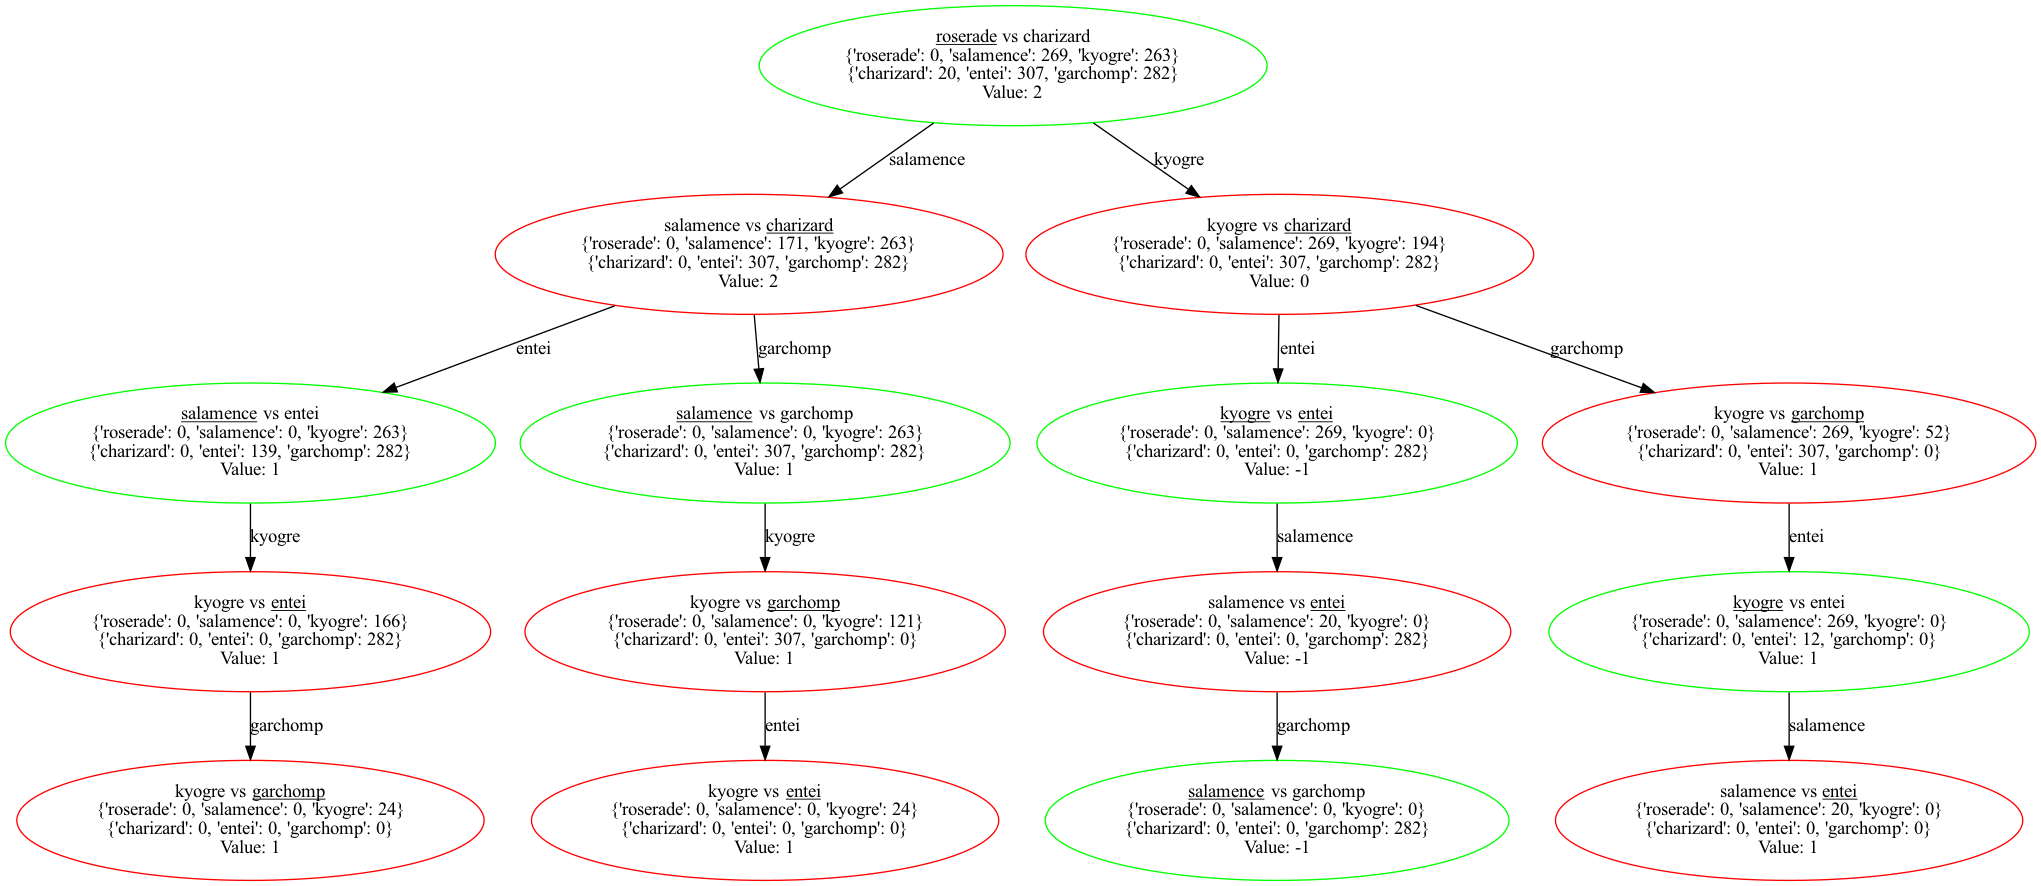
\includegraphics[width=0.9\textwidth]{images/MinMaxTree.png}
	\caption{Possible end game scenario}
	\label{fig:game-plan}
\end{figure}
Figure \ref{fig:game-plan} shows a possible end-game scenario. In this simple example, we assume both players to each
have three Pokémon with full \ac{HP} and no status conditions. Each circle represents two Pokémon battling each other.
Therefore, the circle in the top center indicates, that our \textit{Roserade} is currently fighting against the enemy
\textit{Charizard}. As \textit{Charizard} is a \textit{Fire}-type Pokémon which has a type advantage against his enemy,
our \textit{Roserade} will faint in this matchup, indicated by the underlined name. This means, that now Player 1 has to
switch in a new Pokémon. A green circle around a node indicates that the first player has to make a turn as his 
Pokémon fainted, and a red circle marks a decision for Player 2. The first line below the names of the two opposing
Pokémon displays the amount of \ac{HP} the first team has left after this battle took place. As \textit{Roserade} fainted,
it has zero \ac{HP} left whereas the other two Pokémon in his team are still at full health. Below that, the remaining 
\ac{HP} of the second team is displayed. \textit{Charizard} is \textit{expected} to survive the battle with an 
\textit{expected} amount of 141 \ac{HP} remaining. Next, we have two possible options remaining, we can either send
\textit{Kyogre} or \textit{Azumarill} to defeat the enemy \textit{Charizard}. Taking a look at the leaves of the tree,
the \textit{value} of a leaf node is \textit{- 1} if the enemy wins the battle and \textit{1} if we win the battle. 
The value of a non-leaf node is the sum of the values of the children nodes. The \textit{value} of two means that we 
expect to win the battle. As a result of this, the best choice in our example scenario is to use \textit{Azumarill} to 
defeat the already damaged \textit{Charizard}. \\
\todo{Explain why MinMax Tree is correct. Pokemon don't have expected items / moves!}

\subsection{Determining matchups}
\label{sec:determine-matchups}
In order to determine whether to attack or to switch, we need to determine how the optimal moves for a Pokémon against
another Pokémon are calculated. As stated before, the amount of possible combinations combined with the non-deterministic
nature of the game makes it unfeasible get the optimal move combination by simulating every possible combination of 
actions and reactions over the span of multiple turns. Therefore, we determine the optimal moves for a Pokémon using 
this simplified method: \\
We start by generating all possible move combinations for a Pokémon with a given length. Then, we simulate the outcome
of the battle, if the attacking Pokémon would use these moves in the defined order given the enemy would not do anything
\footnote{The option of not doing anything in a turn does not exist in Pokémon, if possible, the player is always 
forced to either select a move or switch.} Here, we also take boosting, items, status effects and the possibly changing
field state into account \todo{Reference to further work with things that do not work like recognizing focus items}.
In the early game. Then, the combination resulting in the lowest amount of turns until the enemy faints is selected. 
It is important to note that this is not necessarily the move that the bot will use in the next turn as in the 
\textit{Discover}-Phase healing, status and other beneficial effects are prioritized.